\documentclass{beamer}

\usepackage[utf8]{inputenc}

\usepackage{alltt}
\usepackage{xcolor}

\usepackage{tikz}
\usetikzlibrary{arrows,petri,topaths}
\usepackage{tkz-berge}

%% Colors for source highlighting
\definecolor{scKW}  {HTML}{AA37F2}
\definecolor{scFct} {HTML}{1010FF}
\definecolor{scType}{HTML}{228B22}
\definecolor{scVar} {HTML}{A45936}
\definecolor{scComm}{HTML}{B32525}

%% Define _s_cala commands
\newcommand{\sK}[1]{{\color{scKW} #1}}
\newcommand{\sF}[1]{{\color{scFct} #1}}
\newcommand{\sV}[1]{{\color{scVar} #1}}
\newcommand{\sT}[1]{{\color{scType} #1}}
\newcommand{\sC}[1]{{\color{scComm} #1}}
\newcommand{\sH}[1]{{\color{white} #1}}
\newcommand{\sS}{\vspace{0.8mm}}

%% Define other commands
\newcommand{\KW}{\textbf}

\setbeamercovered{transparent}
\setbeamertemplate{navigation symbols}

\title{FlowPools}
\subtitle{A Lock-Free Deterministic Concurrent Dataflow Abstraction}

\author{Tobias Schlatter\inst{1} \and Aleksandar Prokopec\inst{2} \and
  Heather Miller\inst{2} \and  Philipp Haller\inst{2} \and Martin
  Odersky\inst{2}}
\date{June 21, 2012}
\institute{\inst{1}Student, EPFL \and \inst{2}Advisors, LAMP, EPFL}

\begin{document}

\begin{frame}
  \titlepage
\end{frame}

\section{Introduction}
\begin{frame}
  \frametitle{Outline}
  
  \begin{block}{What is a FlowPool}\end{block}
  \begin{block}{Implementation}\end{block}
  \begin{block}{Multi-Lane FlowPools}\end{block}
  \begin{block}{Benchmarks}\end{block}

\end{frame}

\begin{frame}
  \frametitle{What is a FlowPool}
  \framesubtitle{Big Picture}

  \begin{block}{Collection}
    \begin{itemize}
    \item Deterministic
    \item Lock-Free
    \item Asynchronous
    \item Unordered
    \end{itemize}
  \end{block}

  \pause

  \begin{block}{Determinism}
    Every execution of a given program with given input eventually
    \begin{itemize}
    \item Always reaches the same state
    \item[] \qquad or
    \item Always fails
    \end{itemize}
  \end{block}

\end{frame}

\begin{frame}
  \frametitle{What is a FlowPool}
  \framesubtitle{Programming Model}

  \begin{block}{Elementary Operations}
    \begin{alltt} \small
      \sK{def} \sF{<<}(\sV x: \sT T): \sT{FlowPool[T]}\sS\\
      \pause
      \sK{def} \sF{seal}(\sV{size}: \sT{Int}): \sT{Unit}\sS\\
      \pause
      \sK{def} \sF{aggregate}[\sT S](\sV{zero}: \sT{=>S})(\sV{cmb}: \sT{(S, S) => S})\\
      \sH{def aggregate[S]}(\sV{folder}: \sT{(S, T) => S}): \sT{Future[S]}
    \end{alltt}
  \end{block}   
  \pause
  \begin{block}{Higher Level Operations}
    \begin{alltt} \small
      \sK{def} \sF{foreach}[\sT U](\sV f: \sT{T => U}): \sT{Future[Unit]}\sS\\
      \sK{def} \sF{++}[\sT{S >: T}](\sV{that}: \sT{FlowPool[S]}): \sT{FlowPool[S]}\sS\\
      \sK{def} \sF{filter}(\sV p: \sT{T => Boolean}): \sT{FlowPool[T]}\sS\\
      \sK{def} \sF{map}[\sT S](\sV f: \sT{T => S}): \sT{FlowPool[S]}\sS\\
      \sK{def} \sF{flatMap}[\sT S](\sV f: \sT{T => FlowPool[S]}): \sT{FlowPool[S]}\sS\\
      \sK{def} \sF{iterate}[\sT T](\sV{start}: \sT T, \sV{len}: \sT{Int})(\sV f: \sT{(T) => T}): \sT{FlowPool[T]}
    \end{alltt}
  \end{block}

\end{frame}

\begin{frame}
  \frametitle{What is a FlowPool}
  \framesubtitle{Flow Graph}

  \centering
  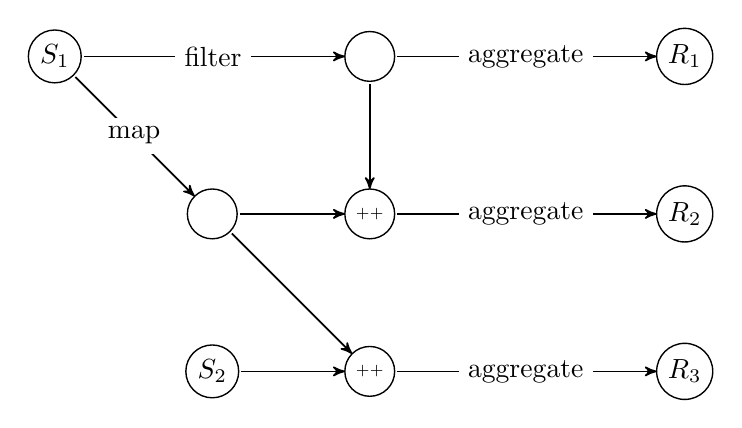
\begin{tikzpicture}[ node distance = 2cm ]
    \tikzset{EdgeStyle/.style={post}}       % directed edges

    \Vertex[x =  0, y =  4, L = $S_1$]{S1}
    \Vertex[x =  2, y =  0, L = $S_2$]{S2}

    \pause

    \Vertex[x =  4, y =  4, L = { }]{S1F}
    \Edge[label = filter](S1)(S1F)

    \pause

    \Vertex[x =  8, y =  4, L = $R_1$]{R1}
    \Edge[label = aggregate](S1F)(R1)

    \pause

    \Vertex[x =  2, y =  2, L = { }]{S1M}
    \Vertex[x =  4, y =  0, L = {\tiny++} ]{AG1}
    \Edge(S1M)(AG1)
    \Edge(S2)(AG1)
    \Edge[label = map](S1)(S1M)

    \pause

    \Vertex[x =  8, y =  0, L = $R_3$]{R3}
    \Edge[label = aggregate](AG1)(R3)

    \pause

    \Vertex[x =  4, y =  2, L = {\tiny++} ]{AG2}
    \Vertex[x =  8, y =  2, L = $R_2$]{R2}

    \Edge[label = aggregate](AG2)(R2)

    \Edge(S1M)(AG2)
    \Edge(S1F)(AG2)

    %\tikzset{EdgeStyle/.append style = {bend right}}

  \end{tikzpicture}  

\end{frame}

\begin{frame}
  \frametitle{Implementation}
  \framesubtitle{Basic Structure}

  \begin{center}
    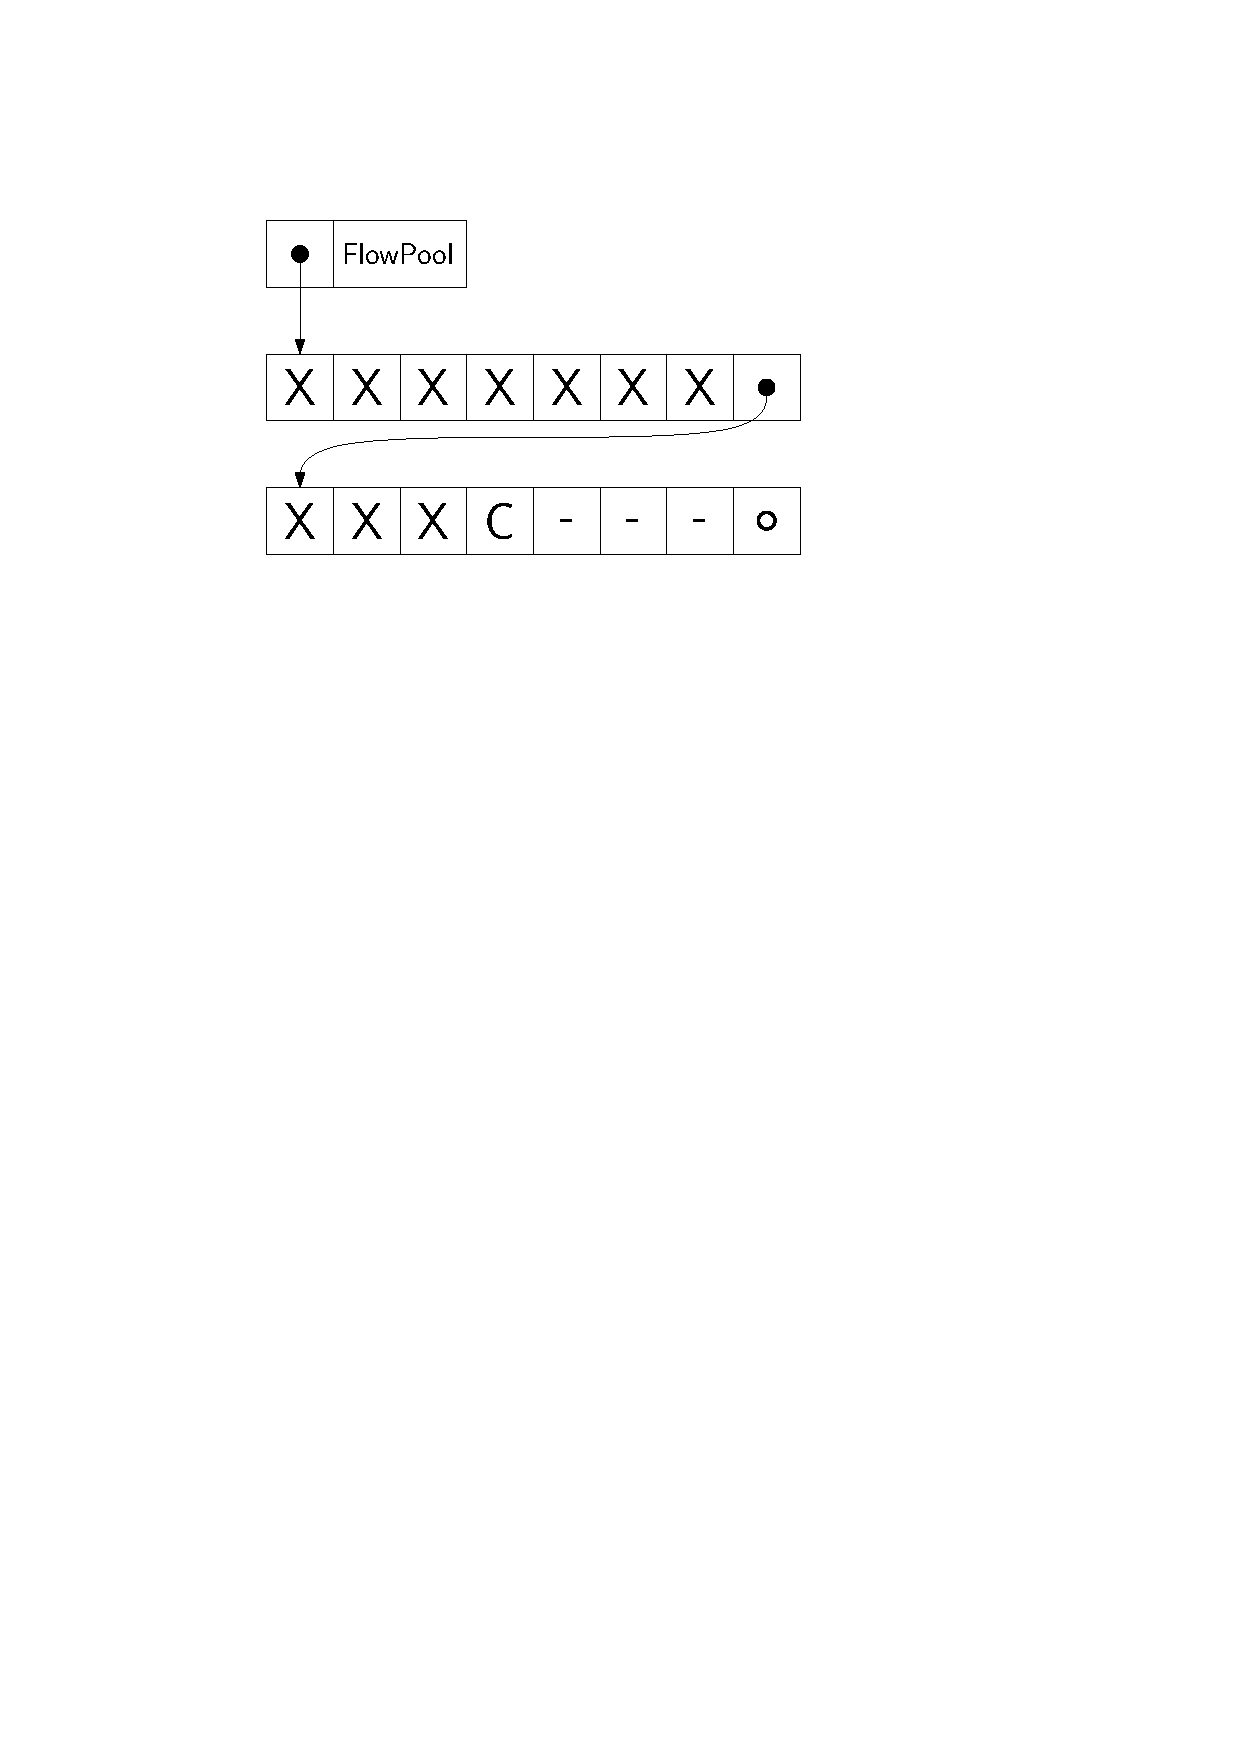
\includegraphics{figs/SLFP}
  \end{center}

\end{frame}

\begin{frame}
  \frametitle{Implementation}
  \framesubtitle{Some preliminaries}

  \begin{block}{Compare and Swap}
    \texttt{CAS(var, old\_value, new\_value)}
  \end{block}

  \begin{block}{Lock-Freedom}
    Show algorithm using only CAS that is not lock-free. (live-lock?)
    % TODO
  \end{block}

\end{frame}

\begin{frame}
  \frametitle{Implementation}
  \framesubtitle{Insert}

  \begin{center}
    \includegraphics<1>[page=1]{figs/SLFP_insert}
    \includegraphics<2>[page=2]{figs/SLFP_insert}
    \includegraphics<3>[page=3]{figs/SLFP_insert}
    \includegraphics<4>[page=4]{figs/SLFP_insert}
    \includegraphics<5>[page=5]{figs/SLFP_insert}
    \includegraphics<6>[page=6]{figs/SLFP_insert}
    \includegraphics<7>[page=7]{figs/SLFP_insert}
  \end{center}

  \begin{alltt} \small
    \alert<1-3>{do \{ curo = block(i) \} while (isElem(curo) \&\& i++)}\\
    \alert<4>  {next = block(i+1)}\\
    \alert<4>  {curo = block(i)}\\
                check(curo)\\
    \alert<5>  {if (!CAS(block(i + 1), next, curo)) retry()}\\
    \alert<6>  {if (!CAS(block(i), el, curo)) retry()}\\
    \alert<7>  {invokeCallbacks(el, next)}
  \end{alltt}

\end{frame}

\begin{frame}
  \frametitle{Implementation}
  \framesubtitle{Seal}

  \begin{center}
    \includegraphics<1>[page=1]{figs/SLFP_seal}
    \includegraphics<2>[page=2]{figs/SLFP_seal}
    \includegraphics<3>[page=3]{figs/SLFP_seal}
    \includegraphics<4>[page=4]{figs/SLFP_seal}
  \end{center}

  \begin{alltt} \small
    \alert<2>  {do \{ curo = block(i) \} while (isElem(curo) \&\& i++)}\\
    \alert<3>  {if (isSeal(curo) || sealsize < i) error()}\\
    \alert<4>  {s = Seal(sealsize, curo)}\\
    \alert<4>  {if (!CAS(block(i), s, curo)) retry()}\\
  \end{alltt}

\end{frame}

\begin{frame}
  \frametitle{Multi-Lane FlowPools}
  \framesubtitle{Overview}

  \begin{block}{Single-Lane FlowPools: Issues}
    \begin{itemize}
    \item Bad scaling
    \item Like Java's concurrent queues
    \end{itemize}
  \end{block}

  \begin{block}{Solution}
    \begin{itemize}
    \item Extend to multiple lanes
    \item Scales nicely
    \end{itemize}
  \end{block}

\end{frame}

\begin{frame}
  \frametitle{Multi-Lane FlowPools}
  \framesubtitle{Basic Structure}
  \begin{center}
    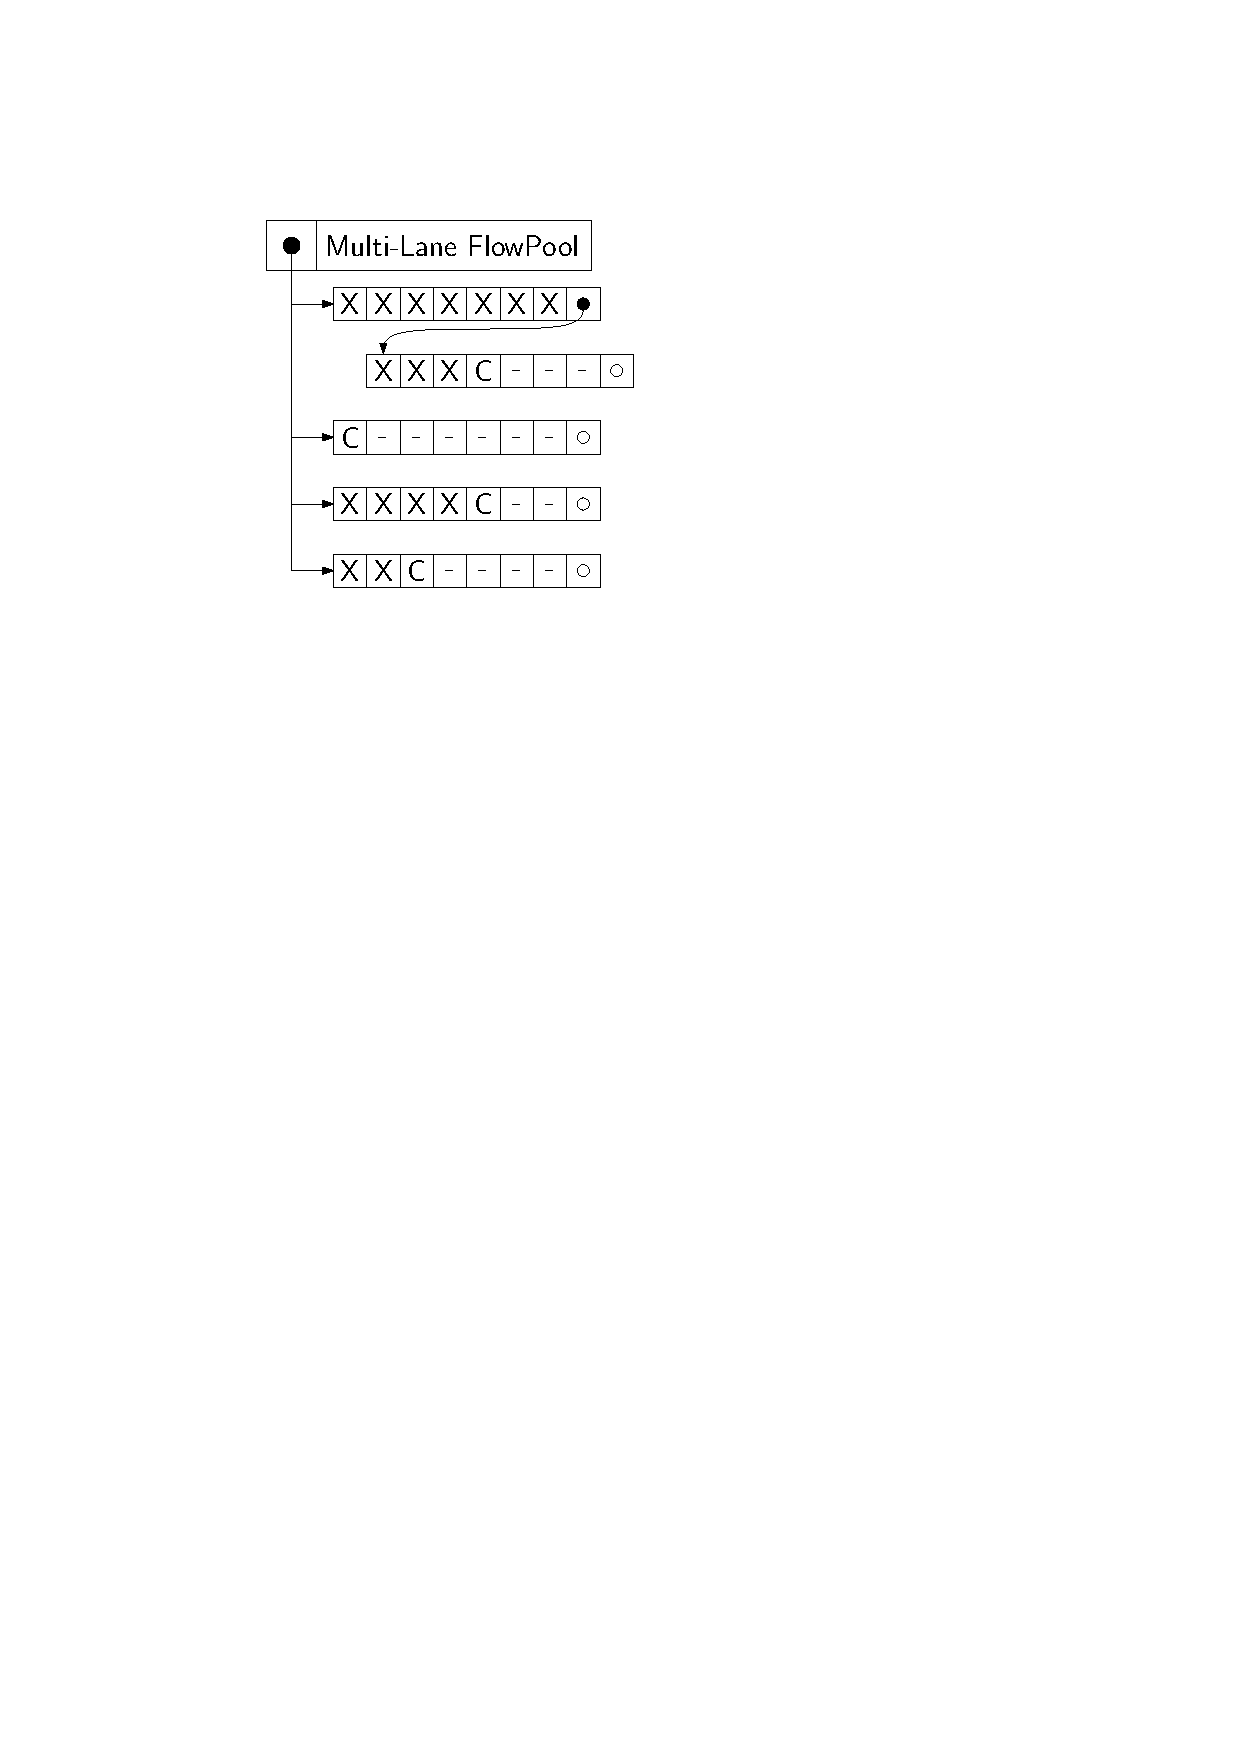
\includegraphics{figs/MLFP}
  \end{center}
\end{frame}

\begin{frame}
  \frametitle{Multi-Lane FlowPools}
  \framesubtitle{Implementational Details}

  \begin{block}{Choice of Lane}
    \begin{enumerate}
    \item $L_{id} = T_{id} \bmod L_{tot}$
    \item $L_{id} = hash(T_{id} + C) \bmod L_{tot}$
    \item Exhaustive search
    \end{enumerate}
  \end{block}

  \begin{block}{Aggregate / Foreach}
    \begin{itemize}
    \item One for each lane
    \item Aggregate at end
    \end{itemize}
  \end{block}

\end{frame}

\begin{frame}
  \frametitle{Multi-Lane FlowPools}
  \framesubtitle{Seal}

- show the difficulties of seal by going into the details of its implementation - feel free to spend several minutes with an animation if necessary

\end{frame}

\begin{frame}
  \frametitle{Benchmarks}

- benchmarks
\end{frame}

\begin{frame}
- conclusion
\end{frame}


\end{document}

%%% Local Variables: 
%%% mode: latex
%%% TeX-master: t
%%% End: 
